\documentclass[usenames,dvipsnames]{beamer}
%
% Choose how your presentation looks.
%
\usepackage[T1]{fontenc}
\usepackage[utf8]{inputenc}
\usepackage{lmodern}  
\usepackage{tikz}%boxy s vysvetlivkami 
\usetikzlibrary{calc}
\usepackage{amsmath}
\usepackage{bm}
\usepackage{color}
\usepackage{listings}

\newcommand{\mytikzmark}[2]{%
  \tikz[remember picture,inner sep=0pt,outer sep=0pt,baseline,anchor=base] 
    \node (#1) {\ensuremath{#2}};}
%    
\newcommand*\circled[1]{\tikz[baseline=(char.base)]{
    \node[shape=circle,draw=Red,inner sep=2pt] (char) {#1};}}
%
\newcommand*\circledd[1]{\tikz[baseline=(char.base)]{
    \node[shape=circle,draw=ProcessBlue, dashed, inner sep=2pt] (char) {#1};}}
%
% For more themes, color themes and font themes, see:
% http://deic.uab.es/~iblanes/beamer_gallery/index_by_theme.html
%
\mode<presentation>
{
  \usetheme{Darmstadt}      % or try Darmstadt, Madrid, Warsaw, ...
  \usecolortheme{default} % or try albatross, beaver, crane, ...
  \usefonttheme{serif}  % or try default, serif, structurebold, ...
  \setbeamertemplate{navigation symbols}{}
  \setbeamertemplate{caption}[numbered]
  \setbeamertemplate{headline}{}
} 
%
%
\title[Block 4]{Block 4\\ Instrumental variable regression (IVR)\\ Two stage least squares (2SLS)\\Simultaneous Equation Models}
\author{Advanced econometrics 1 4EK608 \\Pokročilá ekonometrie 1 4EK416}
\institute{Vysoká škola ekonomická v Praze}
\date{}

\begin{document}
 
\begin{frame}
  \titlepage
\end{frame}

% Uncomment these lines for an automatically generated outline.
\begin{frame}{Outline}
  \tableofcontents
\end{frame}

%---------------------------------------------
\section{Introduction \& repetition from BSc courses}
\begin{frame}{Introduction: endogenous regressors}
\begin{itemize}
\item  CS model: $y_i= \bm{x}_i\bm{\beta}+u_i$ ~~~and~~~ $E[\bm{x}_i, u_i] \neq 0$.
\begin{itemize}
\item If important regressors cannot be measured (thus make part of $u_i$)
and are correlated with observed regressors of LRM.
\item Endogeneity can be caused by measurement errors.
\item Always present in simultaneous equations models (SEMs).
\end{itemize}
\item With endogenous regressors, OLS is biased \& inconsistent.
\end{itemize}
\medskip
Endogeneity in regressors can sometimes be solved
\begin{itemize}
\item By means of proxy variables (if uncorrelated to $u_i$).
\item More detailed (multi-equation) specification, if possible.
\item Using panel data methods (data availability permitting).
\item Using instrumental variable regression (IVR) \\(we need ``good'' instruments, assumptions apply).
\end{itemize}
\end{frame}
%---------------------------------------------
\begin{frame}{Introduction: instrumental variables}
\textbf{Example}:  $\log(\textit{wage}_{\,i})=\beta_0+\beta_1 \textit{educ}_{\,i}+ [\textit{abil}_{\,i} + u_i]$  \\
\vspace{0.3cm}
\textbf{Instrumental variables}
\begin{enumerate}
\item Not in the main (structural) equation: no effect on the dependent variable after controlling for observed regressors.
\item Correlated (positively or negatively) with the endogenous regressor  (this can be tested).
\item Not correlated with the error term (in some cases, this can be tested, see Sargan test discussed next).
\end{enumerate}
\bigskip
\begin{itemize}
\item Possible IVs: father's education, mother's education, number of siblings, etc.\\ 
\smallskip
Usually, $\textit{IQ}$ is not a good IV - it's often correlated with $\textit{abil}$, i.e. with the error term $[\textit{abil}_{\,i} + u_i]$.
\end{itemize}
\end{frame}
%---------------------------------------------
\section{Instrumental variables}
\begin{frame}{Instrumental variables}
\begin{itemize}
    \item $y_i = \beta_0 + \beta_1 x_i + u_i$ \qquad SLRM with exogenous regressor $x$:
    $$
    \begin{matrix}
    y & \leftarrow & x \\
      & \nwarrow & \\
      & & u
    \end{matrix}
    \qquad \qquad \textnormal{and} \qquad
    \frac{\textnormal{d} \, y}{\textnormal{d} \, x} = \beta_1 = \frac{\textnormal{cov}(y,x)}{\textnormal{var}(x)}
    $$
    ~\\
    \item $y_i = \bm{x}_i \bm{\beta} + u_i$ \qquad MLRM with exogenous regressor(s):
    \begin{align*}
    \bm{\hat{\beta}} &= (\bm{X}^{\prime}\bm{X})^{-1} \bm{X}^{\prime}\bm{y} &|~ \textnormal{subs. for~} \bm{y} \\
    \bm{\hat{\beta}} &= (\bm{X}^{\prime}\bm{X})^{-1} \bm{X}^{\prime}(\bm{X \beta} + \bm{u}) &|~ \textnormal{rearr. \& take expects.} \\
    E[\bm{\hat{\beta}}] &= \bm{\beta} + E[(\bm{X}^{\prime}\bm{X})^{-1} \bm{X}^{\prime}\bm{u}] = \bm{\beta}
    \end{align*}
    \item With exogenous regressors, OLS is unbiased.
\end{itemize}
\end{frame}
%---------------------------------------------
\begin{frame}{Instrumental variables}
\begin{itemize}
    \item $y_i = \beta_0 + \beta_1 x_i + u_i$ \qquad SLRM with endogenous regressor $x$:
    $$
    \begin{matrix}
    y & \leftarrow & x \\
      & \nwarrow & | \\
      & & u
    \end{matrix}
    \qquad \qquad \textnormal{and} \qquad
    \frac{\textnormal{d} \, y}{\textnormal{d} \, x} = \beta_1 + \frac{\textnormal{d} \, u}{\textnormal{d} \, x}
    $$
    ~\\
    \item $y_i = \bm{x}_i \bm{\beta} + u_i$ \qquad MLRM with endogenous regressor(s):
    \begin{align*}
    \bm{\hat{\beta}} &= (\bm{X}^{\prime}\bm{X})^{-1} \bm{X}^{\prime}\bm{y} &|~ \textnormal{subs. for~} \bm{y} \\
    \bm{\hat{\beta}} &= (\bm{X}^{\prime}\bm{X})^{-1} \bm{X}^{\prime}(\bm{X \beta} + \bm{u}) &|~ \textnormal{rearr. \& take expects.} \\
    E[\bm{\hat{\beta}}] &= \bm{\beta} + E[(\bm{X}^{\prime}\bm{X})^{-1} \bm{X}^{\prime}\bm{u}] \neq \bm{\beta}
    \end{align*}
    \item With endogenous regressors, $E[(\bm{X}^{\prime}\bm{X})^{-1} \bm{X}^{\prime}\bm{u}] \neq \bm{0}$. \\Thus, OLS is biased (and asymptotically biased).
\end{itemize}
\end{frame}
%---------------------------------------------
\begin{frame}{Instrumental variables}
\begin{itemize}
    \item $y_i = \beta_0 + \beta_1 x_i + u_i$ \qquad IVR principle (SLRM):
    $$
    \begin{matrix}
    y & \leftarrow & x & \leftarrow & z \\
      & \nwarrow & | & &\\
      & & u & &
    \end{matrix}
    \qquad \qquad \textnormal{and} \qquad
   \beta_1 = \frac{\textnormal{cov}(z,y)}{\textnormal{cov}(z,x)}
    $$
    \item $y_i = \bm{x}_i \bm{\beta} + u_i$ \qquad IVR in MLRMs:
    \begin{align*}
    \bm{\hat{\beta}}_{\textnormal{OLS}} &= 
    (\bm{X}^{\prime}\bm{X})^{-1} \bm{X}^{\prime}\bm{y} \\
    \bm{\hat{\beta}}_{\textnormal{IV}} &= 
    (\bm{Z}^{\prime}\bm{X})^{-1} \bm{Z}^{\prime}\bm{y}
    \end{align*}
    where $\bm{Z}$ is a matrix of instruments, same dimensions as $\bm{X}$.
    \small{
    \begin{itemize}
        \item Exact identification: \# endogenous regressors~ =~ \# IVs,
        \item $\bm{Z}$ follows from $\bm{X}$, each endogenous regressor (column) is replaced by unique instrument (full column ranks of $\bm{X}$,$\bm{Z}$),
        \item in IVR, $R^2$ has no interpretation (SST $\neq$ SSE + SSR),
        \item for IVR, we use specialized robust standard errors,
        \item \textbf{IVR estimator is biased and consistent.}
    \end{itemize}
    }
\end{itemize}
\end{frame}
%---------------------------------------------
\begin{frame}{Instrumental variables: IVR as MM estimator}
Exogenous regressors:
\medskip
\begin{itemize}
    \item MM: replace $E[\bm{X}^{\prime}(\bm{y}-\bm{X\beta})]=\bm{0}$ by $\frac{1}{n}[\bm{X}^{\prime}(\bm{y}-\bm{X\hat{\beta}})]=\bm{0}$\\and solve moment equations
    \medskip
    \item OLS provides identical estimate: $\bm{\hat{\beta}}_{\textnormal{OLS}} = (\bm{X}^{\prime}\bm{X})^{-1} \bm{X}^{\prime}\bm{y} $
\end{itemize}
\bigskip
With endogenous regressors (exact identification), moment conditions change:
\medskip
\begin{itemize}
    \item MM: replace $E[\bm{Z}^{\prime}(\bm{y}-\bm{X\beta})]=\bm{0}$ by $\frac{1}{n}[\bm{Z}^{\prime}(\bm{y}-\bm{X\hat{\beta}})]=\bm{0}$\\and solve moment equations
    \medskip
    \item IVR provides identical estimate: $\bm{\hat{\beta}}_{\textnormal{IV}} = (\bm{Z}^{\prime}\bm{X})^{-1} \bm{Z}^{\prime}\bm{y} $
\end{itemize}

\end{frame}
%---------------------------------------------
\begin{frame}{Instrumental variables: IVR as MM estimator}

$y_{i1}=\beta_0 + \beta_1 y_{i2} + \beta_2 x_{i2} + \dots + \beta_k x_{ik} + u_{i} \quad|~z_1 \textnormal{~ is IV for } y_2$\\
\begin{align*}
n^{-1} \sum_{i=1}^n ~~~~~~(y_{i1}-\hat{\beta}_0-\hat{\beta}_1 y_{i2}-\hat{\beta}_2 x_{i2}- \dots- \hat{\beta}_k x_{ik})&=0 \\
n^{-1} \sum_{i=1}^n \, \textcolor{red}{z_{i1}} \cdot (y_{i1}-\hat{\beta}_0-\hat{\beta}_1 y_{i2}-\hat{\beta}_2 x_{i2}- \dots- \hat{\beta}_k x_{ik})&=0 \\
n^{-1} \sum_{i=1}^n \, \textcolor{blue}{x_{i2}} \cdot (y_{i1}-\hat{\beta}_0-\hat{\beta}_1 y_{i2}-\hat{\beta}_2 x_{i2}- \dots- \hat{\beta}_k x_{ik})&=0 \\
       & \dots \\
n^{-1} \sum_{i=1}^n \, \textcolor{blue}{x_{ik}} \cdot (y_{i1}-\hat{\beta}_0-\hat{\beta}_1 y_{i2}-\hat{\beta}_2 x_{i2}- \dots- \hat{\beta}_k x_{ik})&=0
\end{align*} 
\vspace{-0.5cm}
\begin{itemize}
    \item In moment equations, $y_{i2}$ is replaced by $z_{i1}$
    \item Exogenous regressors serve as their own instruments.
\end{itemize}
\end{frame}
%---------------------------------------------
\begin{frame}{IVR estimator is consistent}
\begin{align*}
    \bm{\hat{\beta}}_{\textnormal{IV}} &= (\bm{Z}^{\prime}\bm{X})^{-1} \bm{Z}^{\prime}\bm{y} &|~ \textnormal{subs. for~} \bm{y} \\
     \bm{\hat{\beta}}_{\textnormal{IV}} &= (\bm{Z}^{\prime}\bm{X})^{-1} \bm{Z}^{\prime}(\bm{X \beta} + \bm{u}) &|~ \textnormal{rearrange} \\
    \bm{\hat{\beta}}_{\textnormal{IV}} &= \bm{\beta} + (\bm{Z}^{\prime}\bm{X})^{-1} \bm{Z}^{\prime}\bm{u}
    \end{align*}
\begin{itemize}
    \medskip
    \item If consistency condition holds: $\textnormal{plim}\left[\frac{1}{n}\bm{Z}^{\prime}\bm{u}\right]= \bm{0}$, \\$\bm{\hat{\beta}}_{\textnormal{IV}}$ is consistent.
    \medskip
    \item This can be seen from expansion of $[(\bm{Z}^{\prime}\bm{X})^{-1} \bm{Z}^{\prime}\bm{u}] $:
    $$
    \bm{\hat{\beta}}_{\textnormal{IV}} = \bm{\beta} + (n^{-1}\bm{Z}^{\prime}\bm{X})^{-1}\, n^{-1}\bm{Z}^{\prime}\bm{u}
    $$
\end{itemize}
\end{frame}
%---------------------------------------------
\begin{frame}{Instrumental variables: over-identification}
\vspace{-0.5cm}
$$y_{i1}=\beta_0 + \beta_1 y_{i2} + \beta_2 x_{i2} + \dots + \beta_k x_{ik} + u_{i} \quad|~z_1, z_2, z_3 \textnormal{~ are IVs for } y_2$$

\begin{itemize}
    \item By choosing any of the $z_1, z_2, z_3$ IVs \\(or any linear combination of), we perform IVR
    \item $\hat{\bm{\beta}}_{\textnormal{\,IV}}$ values change, as IV  in moment equations changes.
    \item We cannot ``simply'' use all three instruments. \\If \# columns in $\bm{Z}$ ($l$) ~>~ \# columns in $\bm{X}$ ($k$),\\
    $\bm{Z}^{\prime}\bm{X}$ is $(l\times k)$ with rank $k$ and no inverse:
    \\$\bm{\hat{\beta}}_{\textnormal{IV}} = (\bm{Z}^{\prime}\bm{X})^{-1} \bm{Z}^{\prime}\bm{y}$ cannot be calculated \\
    \medskip
    \item Solution: Project $\bm{X}$ to the space column of $\bm{Z}$ (GMM).\\
    ($\bm{X}$ has an endogenous column, $\bm{Z}$ is purely exogenous).
\end{itemize}
\end{frame}
%---------------------------------------------
\begin{frame}{Instrumental variables: over-identification}
\begin{block}{Projection matrices (exogenous $\bm{X}$) -- repetition}
\vspace{-0.5cm}
\begin{align*} 
\hat{\bm{y}} & = \bm{X}\hat{\bm{\beta}} =  
\bm{X}(\bm{X}^{\prime}\bm{X})^{-1} \bm{X}^{\prime}\bm{y} = \bm{Py}\\
\bm{y} & = \hat{\bm{y}} + \hat{\bm{u}} = \bm{Py} + \bm{My}, \textnormal{~where} \\
\bm{M} & = \bm{I}  - \bm{X}(\bm{X}^{\prime}\bm{X})^{-1} \bm{X}^{\prime} = \bm{I} - \bm{P}
\end{align*}
\end{block}
\begin{itemize}
    \item Projection of columns of $\bm{X}$ in the column space of $\bm{Z}$:
$$
\hat{\bm{X}} = 
\bm{Z}(\bm{Z}^{\prime}\bm{Z})^{-1} \bm{Z}^{\prime}\bm{X} = \bm{P}_{\bm{Z}}\bm{X},
$$
\item Columns of $\hat{\bm{X}}$ are linear combinations of columns in $\bm{Z}$. 
\medskip 
\item Exogenous columns in $\bm{X}$ are repeated in $\bm{Z}$, hence projected on themselves \& therefore do not change between $\bm{X}$ and $\bm{Z}$.
\medskip
\item General form of the IV estimator (over-identification):
\begin{align*}
 \bm{\hat{\beta}}_{\textnormal{IV}} &= (\hat{\bm{X}}^{\prime}\bm{X})^{-1} \hat{\bm{X}}^{\prime}\bm{y}
\end{align*}
\end{itemize}
\end{frame}
%---------------------------------------------
\begin{frame}{Instrumental variables: over-identification}
\begin{itemize} 
    \item Projection of columns of $\bm{X}$ in the column space of $\bm{Z}$:
$$
\hat{\bm{X}} = 
\bm{Z}(\bm{Z}^{\prime}\bm{Z})^{-1} \bm{Z}^{\prime}\bm{X},
$$
\item It may be shown that IVR is equivalent to OLS regression \\$\bm{y} \leftarrow \hat{\bm{X}}$:
\begin{align*}
 \bm{\hat{\beta}}_{\textnormal{IV}} &= 
 (\hat{\bm{X}}^{\prime}\bm{X})^{-1} \hat{\bm{X}}^{\prime}\bm{y} \\
 &= (\bm{X}^{\prime}(\bm{I}-\bm{M}_Z)\bm{X})^{-1} \bm{X}^{\prime}(\bm{I}-\bm{M}_Z)\bm{y} \\
 &= (\hat{\bm{X}}^{\prime}\hat{\bm{X}})^{-1} \hat{\bm{X}}^{\prime}\bm{y}
\end{align*}
\item $\bm{y} \leftarrow \hat{\bm{X}}$ is part of a two-stage LS (2SLS) method, \\(discussed next).
\end{itemize}
\end{frame}
%---------------------------------------------
\begin{frame}{Instrumental variables: identification conditions}
\begin{itemize} 
\item In $\bm{y} = \bm{X\beta}+\bm{u}$, multiple $\bm{x}_j$ regressors may be endogenous.
\medskip
\item Identification (estimability) conditions:
\medskip
\begin{itemize} 
\item \textbf{Order condition:} We need at least as many IVs (excluded exogenous variables) as there are included endogenous regressors in the main (structural) equation.  
\\ \medskip This is a necessary condition for identification. 
\bigskip
\item \textbf{Rank condition:} $\hat{\bm{X}} = 
\bm{Z}(\bm{Z}^{\prime}\bm{Z})^{-1} \bm{Z}^{\prime}\bm{X}$ has full column rank $(k)$ so that $(\hat{\bm{X}}^{\prime}\bm{X})^{-1}$ or $(\hat{\bm{X}}^{\prime}\hat{\bm{X}})^{-1}$ can be calculated in the IV estimator $\bm{\hat{\beta}}_{\textnormal{IV}} =  (\hat{\bm{X}}^{\prime}\bm{X})^{-1} \hat{\bm{X}}^{\prime}\bm{y}$ (will be discussed in detail with respect to 2SLS method and for SEM models).
\\ \medskip This is a necessary and sufficient condition for identification. 
\end{itemize}
\end{itemize}
\end{frame}
%---------------------------------------------
\begin{frame}{Instrumental variables: statistical properties}
\textbf{SLRM:} $y_{i1} = \beta_0 + \beta_1 x_{i1} + u_i \quad |~x_{i1} \textnormal{~endog.,~} z_{i1} \textnormal{~exists}$
\bigskip
\begin{itemize}
\item Asymptotic variance of the IV estimator decreases with increasing correlation between $z$ and $x$. 
\medskip
\item IV-related routines \& tests are implemented in R, \dots 
\medskip
\item Both endogenous explanatory variables and IVs can be binary variables.
\medskip
\item $R^2$ can be negative and has no interpretation nor relevance if IVR is used.
\end{itemize}
\end{frame}
%---------------------------------------------
\begin{frame}{Instrumental variables: statistical properties}
\textbf{SLRM:} $y_{i1} = \beta_0 + \beta_1 x_{i1} + u_i \quad |~x_{i1} \textnormal{~endog.,~} z_{i1} \textnormal{~exists}$
\medskip
\begin{itemize}
\item In large samples, IV estimator has approximately normal distribution (MM/GMM properties). 
\medskip
\item For calculation of standard errors, we usually need assumption of homoscedasticity conditional on IV(s).\\ Alternatively, we calculate robust errors. 
\medskip
\item Asymptotic variance of the IV estimator is always higher than  of the OLS estimator. 
$$ \textnormal{var}(\hat{\beta}_{1,IV})=\frac{\hat{\sigma}^2}{\textit{SST}_{x} \cdot R^2_{x,z}} ~~~>~~
\textnormal{var}(\hat{\beta}_{1,OLS})=\frac{\hat{\sigma}^2}{\textit{SST}_x}$$
\end{itemize}
\end{frame}
%---------------------------------------------
\begin{frame}{Instrumental variables: statistical properties}
\textbf{SLRM:} $y_{i1} = \beta_0 + \beta_1 x_{i1} + u_i \quad |~x_{i1} \textnormal{~endog.,~} z_{i1} \textnormal{~exists}$
\medskip
\begin{itemize}
\item If (small) correlation between $u$ and instrument $z$ is possible, inconsistency in the IV estimator can be much higher than in the OLS estimator:
\vspace{0.3cm}
\begin{align*}
\mathrm{plim}\hat{\beta}_{1, OLS} = \beta_1 + \mathrm{corr}(x, u) \cdot \frac{\sigma_u}{\sigma_x} \\
~\\
\mathrm{plim}\hat{\beta}_{1, IV} = \beta_1 + \frac{\mathrm{corr}(z, u)}{\mathrm{corr}(z, x)} \cdot \frac{\sigma_u}{\sigma_x} \\
\end{align*}
\item Weak instrument: if correlation between  $z$ and $x$ is small.
\end{itemize}
\end{frame}
%---------------------------------------------
\begin{frame}{Instrumental variables: statistical properties}
\textbf{MLRM:} $\bm{y} = \bm{X\beta} + \bm{u} \quad |\textnormal{~valid} ~\bm{Z} \textnormal{~exists}$
\medskip
\begin{itemize}
\item IVR method is a ``trick'' for consistent estimation of the ceteris paribus effects, i.e. $\hat{\beta}_{j,\textnormal{IV}}$.
\medskip
\item Fitted values are generated as $\hat{\bm{y}} = \bm{X} \hat{\bm{\beta}}_{\textnormal{IV}}$\\
(NOT from $\hat{\bm{y}} = \hat{\bm{X}} \hat{\bm{\beta}}_{\textnormal{IV}}$).
\medskip
\item Similarly: var$(\hat{u}_i) = \hat{\sigma}^2 = \frac{1}{n-k} \sum_{i=1}^n (y_i - \bm{x}_i \hat{\bm{\beta}}_{\textnormal{IV}})^2$\\d.f. correction is superfluous (asymptotic use only). 
\medskip
\item Asy.Var$(\hat{\bm{\beta}}_{\textnormal{IV}}) = \hat{\sigma}^2
(\bm{Z}^{\prime}\bm{X})^{-1}(\bm{Z}^{\prime}\bm{Z})(\bm{X}^{\prime}\bm{Z})^{-1}
$\\
for the exactly identified \& homoscedastic case.
\medskip
\item With heteroscedasticity and/or over-identification, the Asy.Var$(\hat{\bm{\beta}}_{\textnormal{IV}})$ formula is complex and built into all SW packages.
\end{itemize}
\end{frame}
%---------------------------------------------
\section{Two stage least squares}
\begin{frame}{2SLS as a special case of IVR}
$$
 \bm{\hat{\beta}}_{\textnormal{IV}} ~=~ 
 (\hat{\bm{X}}^{\prime}\bm{X})^{-1} \hat{\bm{X}}^{\prime}\bm{y} 
 ~=~ (\hat{\bm{X}}^{\prime}\hat{\bm{X}})^{-1} \hat{\bm{X}}^{\prime}\bm{y}
$$
\textbf{2SLS}: 
\begin{itemize}
\item Structural equation (as in SEMs) \\
\smallskip
$y_1=\beta_0+\beta_1 y_2+\beta_2 x_2+ \dots + \beta_k x_{k} +u \quad | ~z_1 \textnormal{~exists}$\\
\medskip
\item Reduced form for $y_2$ – endogenous variable as function of all exogenous variables (including IVs) \\
\smallskip
$y_2=\pi_0+\pi_1 z_1 + \pi_{2} x_{2} + \dots +\pi_k x_k + \varepsilon$
\medskip
\item $1^{\textnormal{st}}$ stage of 2SLS: Estimate reduced form by OLS
\smallskip
\begin{itemize}
    \item Order condition for identification of the structural equation: at least one instrument for each endogenous regressor).
    \smallskip
    \item If $z_1$ is an IV for $y_2$, its coefficient must not be zero (rank condition for identification) in the reduced form equation - see stage 2 of 2SLS.
\end{itemize}
\end{itemize}
\end{frame}
%---------------------------------------------
\begin{frame}{2SLS as a special case of IVR}
$$
 \bm{\hat{\beta}}_{\textnormal{IV}} ~=~ 
 (\hat{\bm{X}}^{\prime}\bm{X})^{-1} \hat{\bm{X}}^{\prime}\bm{y} 
 ~=~ (\hat{\bm{X}}^{\prime}\hat{\bm{X}})^{-1} \hat{\bm{X}}^{\prime}\bm{y}
$$
\textbf{2SLS}: 
\begin{itemize}
\item Structural equation\\
\smallskip
$y_1=\beta_0+\beta_1 y_2+\beta_2 x_2+ \dots + \beta_k x_{k} +u \quad | ~z_1 \textnormal{~exists}$\\
\medskip
\item $1^{\textnormal{st}}$ stage of 2SLS: estimate reduced form for $y_2$:\\
\smallskip
$\hat{y}_2=\hat{\pi}_0+\hat{\pi}_1 z_1 + \hat{\pi}_{2} x_{2} + \dots +\hat{\pi}_k x_k$
\medskip
\item $2^{\textnormal{nd}}$ stage of 2SLS: Use $\hat{y}_2$ to estimate structural equation:\\
\smallskip
$y_1=\beta_0+\beta_1 \hat{y}_2 +\beta_2 x_2+ \dots + \beta_k x_{k} +u$
\smallskip
\item Note that RHS in the $2^{\textnormal{nd}}$ stage contains all exogenous regressors repeated from $\bm{X}$, while $\hat{y}_2$ is $y_2$ ``projected'' onto $\bm{Z}$ and thus uncorrelated with $u$.
\item Order condition fulfilled. Rank condition explained: if $\pi_1=0$, $\hat{y}_2$ is a perfect linear combination of the remaining RHS regressors in $2^{\textnormal{nd}}$ stage.
\end{itemize}
\end{frame}
%---------------------------------------------
\begin{frame}{Instrumental variables}
Instrumental variables: summary\\
\vspace{0.3cm}
\begin{itemize}
\item Excluded from the main / structural equation
\item Must be correlated with endogenous regressor(s)
\item Must not be correlated with $u$
\end{itemize}
\vspace{0.3cm}
All IVs used in IVR / 2SLS estimation must fulfill the conditions above.\\
\vspace{0.3cm}
In 2SLS, $1^{\textnormal{st}}$ stage is used to generate the ``best'' IV.\\
With multiple endogenous regressors, reduced forms for each endogenous regressor must be constructed and estimated, rank and order conditions apply.
\end{frame}
%---------------------------------------------
\begin{frame}{Two stage least squares}
\textbf{2SLS properties}
\vspace{0.3cm}
\begin{itemize}
\item The standard errors from the OLS second stage regression are biased and inconsistent estimators with respect to the original structural equation (SW handles this problem automatically).
\vspace{0.3cm}
\item If there is one endogenous variable and one instrument then 2SLS = IVR
\vspace{0.3cm}
\item With multiple endogenous variables and/or multiple instruments, 2SLS is a special case of IVR.\\ \medskip
\footnotesize
Example:\\ Consider MLRM with one endogenous regressor and 3 relevant IVs. Choosing any IV (or any ad-hoc linear combination of IVs) results in IVR (MM-type \& consistent estimator). 2SLS (GMM-type approach) provides the ``best'' IVR estimator -- lowest variance in the $2^{\textnormal{nd}}$ stage comes from best fit between IVs and endogenous regressor in $1^{\textnormal{st}}$ stage.
\vspace{0.3cm}
\end{itemize}
\end{frame}
%---------------------------------------------
\begin{frame}{Two stage least squares}
\textbf{Statistical properties of the 2SLS/IV estimator}
\vspace{0.3cm}
\begin{itemize}
\item Under assumptions completely analogous to OLS, but conditioning on $z_i$ rather than on $x_i$ , 2SLS/IV is consistent and asymptotically normal.
\vspace{0.3cm}
\item 2SLS/IV estimator is typically much less efficient than the OLS estimator because there is more multicollinearity and less explanatory variation in the second stage regression
\vspace{0.3cm}
\item Problem of multicollinearity is much more serious with 2SLS than with OLS
\end{itemize}
\end{frame}
%---------------------------------------------
\begin{frame}{Two stage least squares}
\textbf{Statistical properties of the 2SLS/IV estimator}
\vspace{0.5cm}
\begin{itemize}
\item Corrections for heteroscedasticity/serial correlation analogous to OLS
\vspace{0.3cm}
\item 2SLS/IVR estimamtion easily extends to time series and panel data situations
\end{itemize}
\end{frame}
%---------------------------------------------
\section{IVR diagnostic tests}
\begin{frame}{IVR diagnostic tests: introduction}
LRM: $y_{i1}=\beta_0+\beta_1 y_{i2}+\beta_2 x_{i1}+u_i$; \quad $\bm{z}$ instruments exist \\
\vspace{0.3cm}
\underline{IV regression advantages} for endogenous $y_2$:
\vspace{-0.2cm}
\begin{align*}
& \rightarrow \hat{\beta}_{1,\textnormal{OLS}} \enspace \parbox[t]{24em}{ is a \textcolor{red}{biased and inconsistent estimator} \\(asymptotic errors)}\\
 & \rightarrow \hat{\beta}_{1, \textnormal{IV}} \enspace \parbox[t]{24em}{ is a \textcolor{blue}{biased and consistent estimator} (increased \\sample size (\textit{n}) lowers estimator bias and s.e.)} 
\end{align*}
\underline{IVR disadvantages (price for the IVR)}:
\begin{itemize}
\item $\textnormal{s.e.}(\hat{\beta}_{1, \textnormal{IV}}) > \textnormal{s.e.}(\hat{\beta}_{1,\textnormal{OLS}})$
\item $\hat{\beta}_{1, \textnormal{IV}}$ is biased, even if $y_2$ is actually exogenous\\
\smallskip
$\hat{\beta}_{1, \textnormal{OLS}}$ is unbiased for exogenous regressors \\ 
\small (potentially, pending other G-M conditions).
\end{itemize}
\end{frame}
%---------------------------------------------
\begin{frame}{IVR diagnostic tests: introduction}
LRM: $y_{i1}=\beta_0+\beta_1 y_{i2}+\beta_2 x_{i1}+u_i$; \quad $\bm{z}$ instruments exist
\medskip
\begin{itemize}
\item Is the regressor $y_2$ endogenous / $\mathrm{corr}(y_2, u) \neq 0$ / ? \\
Is it meaningful to use IVR (considering IVRs ``price'')?\\
\textbf{Durbin-Wu-Hausman endogeneity test}\\
\item Are the instruments actually helpful\\
(weakly or strongly correlated with endogenous regressors)? \\
\textbf{Weak instruments test}\\
\item Are the instruments really exogenous / $\mathrm{corr}(z_j, u)=0$ / ?\\
\textbf{Sargan test} (only applicable in case of over-identification)\\
\end{itemize}
\medskip
\small Different types \& specifications for IV-tests exist, often focusing on the distribution of the difference between IVR and OLS estimators ($\bm{\hat{\beta}}_{\textnormal{IV}}-\bm{\hat{\beta}}_{\textnormal{OLS}}$) under the corresponding $H_0$.
\end{frame}
%---------------------------------------------
\begin{frame}{Durbin-Wu-Hausman endogeneity test}
\small 
$$y_{i1}=\beta_0+\beta_1 y_{i2} + \beta_2 x_{i1} +  u_i ~~~~|~z_{i1}, $$
\medskip
\textbf{\underline{DWH test motivation:}} \\If $z_1$ is a proper instrument (uncorrelated with $u$), then $y_2$ is endogenous (correlated with $u$) if and only if $\varepsilon$ (error from reduced form equation) is correlated with $u$. \\
\medskip
\begin{itemize}
\item If $y_2$ is endogenous ~~$\Leftrightarrow ~~\textnormal{corr}(y_2,u)\neq0$
\item Reduced form: $y_2 = \textit{l.f.}(x_1, z_1) + \varepsilon ~\Rightarrow~ y_2 = \hat{y}_2 + \hat{\varepsilon}$
\item $\textnormal{corr}(y_2,u)\neq0 ~\wedge~\textnormal{corr}(\hat{y}_2,u) = 0 ~\Rightarrow~ \textnormal{corr}(\hat{\varepsilon},u)\neq0 $
\item $y_1$ is always correlated with $u$. 
\item Hence, $\hat{\varepsilon}$ is significant in an auxiliary regression\\ \smallskip
$y_{i1}=\beta_0+\beta_1 y_{i2} + \beta_2 x_{i1} + \delta \hat{\varepsilon}_i + u_i$, \\ \smallskip if $y_2$ is an endogenous regressor.
\item IV/IVs being uncorrelated with $u$ is an essential condition for DWH test to ``work''.
\end{itemize}
\medskip
\textbf{\underline{Note:}} other variants of the DWH test exist...
\end{frame}
%---------------------------------------------
\subsection{Durbin-Wu-Hausman (endogeneity in regressors)}
\begin{frame}{Durbin-Wu-Hausman endogeneity test}
Structural equation: 
\begin{align}
\label{eq:one} y_{i1}=\beta_0+\beta_1 y_{i2} + \beta_2 x_{i1} + u_i; \quad \text{IVs: $z_1$ and $z_2$}
\end{align}
Reduced form for $y_2$: 
\begin{align}
\label{eq:two} y_{i2}=\pi_0 + \pi_1 z_{i1} + \pi_2 z_{i2} + \pi_3 x_{i1} + \varepsilon_i
\end{align}
\vspace{-0.4cm}
\begin{itemize}
\item[$H_0$:] $y_2$ is exogenous $\leftrightarrow$ $\hat{\varepsilon}$ is not significant when added to equation \eqref{eq:one}
\item[$H_1$:] $y_2$ is endogenous $\rightarrow$ OLS is not consistent for \eqref{eq:one} estimation, use IVR (2SLS).
\end{itemize}
\textbf{\underline{Testing algorithm:}}
\begin{enumerate}
\item Estimate equation \eqref{eq:two} and save residuals $\hat{\varepsilon}$.
\item Add residuals $\hat{\varepsilon}$ into equation \eqref{eq:one} and estimate using OLS\\ (use HC inference).
\item $H_0$ is rejected if $\hat{\varepsilon}$ in the modified equation \eqref{eq:one} is statistically significant ($t$-test).
\end{enumerate}
\end{frame}
%---------------------------------------------
\subsection{Weak instruments test}
\begin{frame}{Weak instruments}
\textbf{Motivation for Weak instruments and Sargan tests:} \\
\medskip
LRM: \quad $y_{i1}=\beta_0+\beta_1 y_{i2}+\beta_2 x_{i1}+u_i$; \ $z$ instrument exists
\bigskip
\begin{itemize}
\item IVR is consistent if $\mathrm{cov}(z,y_2) \neq 0$ and $\mathrm{cov}(z, u) = 0$
\item If we allow for (weak) correlation between $z$ and $u$, the asymptotic error of IV estimator is:
\small $$\mathrm{plim}(\hat{\beta}_{1, IV}) = \beta_1 + \frac{\mathrm{corr}(z,u)}{\mathrm{corr}(z,y_2)} \cdot \frac{\sigma_u}{\sigma_{y_2}} $$
%BOX
\item If $\mathrm{corr}(z, y_2)$ is too weak (too close to zero in absolute value), OLS may be better than IV. The asymptotic bias for OLS (LRM with endogenous $y_2$):
\small $$\mathrm{plim}(\hat{\beta}_{1,OLS})=\beta_1+\mathrm{corr}(y_2,u) \cdot \frac{\sigma_u}{\sigma_{y_2}}$$
\end{itemize}
Rule of thumb: IF $|\mathrm{corr}(z,y_2)| < |\mathrm{corr}(y_2,u)|$, do not use IVR.
\end{frame}
%---------------------------------------------
\begin{frame}{Weak instruments}
Structural equation: 
\begin{align*}
y_1=\beta_0+\beta_1 y_2 + \beta_2 x_1 + \dots + \beta_{k+1} x_k + u; \quad \text{IVs: $z_1$, $z_2$, \dots , $z_m$}
\end{align*}
The reduced form for $y_2$: 
\begin{align*}
y_2=\pi_0 + \pi_1 x_1 + \pi_2 x_2 + \dots + \pi_k x_k + \theta_1 z_1 + \dots + \theta_m z_m + \varepsilon
\end{align*}
\vspace{-0.3cm}
\begin{itemize}
\item[$H_0$:] $\theta_1=\theta_2=\dots=\theta_m=0$ \\interpretation: ``instruments are weak''.
\item[$H_1$:] $\neg$ $H_0$
\end{itemize}
\bigskip
\textbf{\underline{Testing for weak instruments:}} \\
\medskip
Use $F$-test (heteroscedasticity-robust). \\Note: multiple testing approaches \& exist.
\end{frame}
%---------------------------------------------
\subsection{Sargan (exogeneity in IVs, over-identification only)}
\begin{frame}{Sargan test (over-identification only)}
Structural equation: 
\begin{align}
\label{eq:three} y_{i1}=\beta_0+\beta_1 y_{i2} + \beta_2 x_{i1} + u_i; \quad \text{IVs: $z_1$, $z_2$, \dots}
\end{align}
\vspace{-0.2cm}
\begin{itemize}
\item[$H_0$:] all IVs are uncorrelated with $u$
\item[$H_1$:] at least one instrument is endogenous
\end{itemize}
\bigskip
\textbf{\underline{Testing algorithm:}}
\begin{enumerate}
\item Estimate equation \eqref{eq:three} using IVR and save the $\hat{u}$ residuals.
\item Use OLS to estimate auxiliary regression: \ $\hat{u} \leftarrow f(\bm{x, z})$ and save the $R_a^2$
\item Under $H_0$: $nR_a^2 \sim \chi_q^2$ where \\$q =$ (number of IVs) - (number of endogenous regressors) 
 \\i.e. $q$ is the number of over-identifying variables.
\item If the observed test statistic exceeds its critical value \\(at a given significance level), we reject $H_0$.
\end{enumerate}
\end{frame}
%---------------------------------------------
\begin{frame}[fragile]{IVR diagnostic tests: example}
%\begin{minipage}[t]{.3\textwidth}

\tiny
\begin{lstlisting}[escapechar=\%]
Call:
ivreg(formula = lbwght ~  %\mytikzmark{REG}{packs + male}% |  %\mytikzmark{IV}{faminc + motheduc + male}%, 
    data = bwght)

Residuals:
     Min       1Q   Median       3Q      Max 
-1.66291 -0.09793  0.01717  0.11616  0.82793 

Coefficients:
            Estimate Std. Error t value Pr(>|t|)    
(Intercept)  4.77419    0.01099 434.478  < 2e-16 ***
packs       -0.25584    0.07613  -3.361 0.000798 ***
male         0.02422    0.01048   2.311 0.021003 *  

Diagnostic tests:
                  df1  df2 statistic p-value    
Weak instruments    2 1383    38.732  <2e-16 %\mytikzmark{1}{***}%
Wu-Hausman          1 1383     5.385  0.0205 %\mytikzmark{2}{* }% 
Sargan              1   NA     4.476  0.0344 %\mytikzmark{3}{*  }%
---
Signif. codes:  0 *** 0.001 ** 0.01 * 0.05 . 0.1  

Residual std. error: 0.195 on 1384 d.f.
Multiple R-Squared: -0.04371,	Adj R-sqr: -0.04522 
Wald test: 8.342 on 2 and 1384 DF,  p-value: 0.0002504 
\end{lstlisting}
%\end{minipage}

\begin{tikzpicture}[<-,overlay,remember picture,inner sep=0.6pt,shorten <=0.2em,font=\tiny]
\tikzset{
    mynode/.style={rectangle, draw=Red,fill=white, minimum size=1cm, text width=4.2cm, font=\scriptsize},
    mynode2/.style={rectangle, minimum size=.5cm, text width=3cm},
    mynode3/.style={rectangle, minimum size=.5cm, text width=.5cm},
    myarrow/.style={->, >=stealth, semithick, Red},
    myarrow2/.style={->, >=stealth, semithick, Blue}
}
\node[mynode] at (9,7)(box){Wooldridge, bwght dataset\\ R code, \{AER\} package};
\node[mynode3] at (11,5.5)(box4){IVs};
\node[mynode2] at (10.2,5)(box5){Regressors \\explicitly included \\in equation};
\node[mynode2] at (10.2,3)(box1){\checkmark Reject $H_0$: \\IVs are weak};
\node[mynode2] at (10.2,2)(box2){\checkmark Reject $H_0$: \\pack are exogenous\\(IVR adequate)};
\node[mynode2] at (10.2,1)(box3){!! Reject $H_0$: all IVs \\ are uncorrelated with $u$ \\ (!DWH assumptions!)};
\draw[myarrow] (box1) -- ++ (1);
\draw[myarrow] (box2) -- ++ (2);
\draw[myarrow] (box3) -- ++ (3);
\draw[myarrow2] (box4) -- ++ (IV);
\draw[myarrow2] (box5) -- ++ (REG);
\end{tikzpicture}
\end{frame}
%---------------------------------------------
\section{SEM: introduction}
\begin{frame}{Simlultaneous equation model (SEM)}
    \begin{itemize}
        \item SEM: outline
        \bigskip
        \item SEM: identification
        \bigskip
        \item Identification conditions
        \bigskip
        \item SEMs with more than two equations
    \end{itemize}
\end{frame}
%---------------------------------------------
\begin{frame}{SEM: introduction}
\underline{\textbf{Simultaneity is another important form of endogeneity}}\\
\bigskip
Simultaneity occurs if at least two variables are jointly determined. A typical case is when observed outcomes are the result of separate behavioral mechanisms that are coordinated in an equilibrium. 
\medskip
\\Prototypical case: a system of demand and supply equations:
\begin{itemize}
\item $D(p) $ how high \textit{would} demand be if the price was set to $p$?
\item $S(p) $ how high \textit{would} supply be if the price was set to $p$?
\vspace{0.2cm}
\item Both mechanisms have a ceteris paribus interpretation.
\item Observed quantity and price will be determined in equilibrium, where $D(p)=S(p)$.
\end{itemize}
\medskip
Simultaneous equations systems can be estimated by 2SLS/IVR\\
\dots ~Identification conditions apply.
\end{frame}
%---------------------------------------------
\begin{frame}{SEM examples}
\textcolor{Blue}{Example 1:} Labor supply and demand in agriculture \\
\bigskip
\qquad $h_s  = \alpha_1 w + \beta_1 z_1 + u_1$ \\
\qquad $h_d  = \alpha_2 w + \beta_2 z_2 + u_2$ \\
\begin{itemize}
\item Endogenous variables, exogenous variables, \\observed and unobserved supply shifter, \\observed and unobserved demand shifter\\
\medskip
\item We have $n$ regions, market sets equilibrium price and quantity in each. We observe the equilibrium values only \\
\vspace{0.3cm}
$h_{is} = h_{id} \Rightarrow (h_i, w_i)$
\end{itemize}
\end{frame}
%---------------------------------------------
\begin{frame}{SEM examples}
\textcolor{Blue}{Example 1:} Labor supply and demand in agriculture contnd.\\
\bigskip
\begin{itemize}
\item [] $h_i  = \alpha_1 w_i + \beta_1 z_{i1} + u_{i1}$
\item [] $h_i  = \alpha_2 w_i + \beta_2 z_{i2} + u_{i2}$ \\
\medskip
\item If we have the same exogenous variables in each equation, we cannot identify (distinguish) equations. \\
\medskip
\item We assume independence between errors in structural equations \& exogenous regressors. 
\end{itemize}
\end{frame}
%---------------------------------------------
\begin{frame}{SEM examples}
\textcolor{Blue}{Example 1:} Labor supply and demand in agriculture contnd.\\
\bigskip
If we estimate the structural equation with OLS method, estimators will be biased – so called ``simultaneity bias''. \\
\medskip
\quad \ $y_1  = \alpha_1 y_2 + \beta_1 z_1 + u_1 $ \\
\medskip
\quad \ $y_2  = \alpha_2 y_1 + \beta_2 z_2 + u_2 $ \\
\bigskip
$y_2$ is dependent on $u_1$ \\
(substitute RHS of the $1^{st}$ equation for $y_1$ in the $2^{nd}$ eq.)\\
\medskip
$\Rightarrow y_2  = \bigg[ \frac{\alpha_2 \beta_1}{1-\alpha_2 \alpha_1} \bigg] z_1 + \bigg[ \frac{\beta_2}{1 - \alpha_2 \alpha_1} \bigg] z_2 + \bigg[\frac{\alpha_2 u_1 + u_2}{1-\alpha_2 \alpha_1} \bigg] $ \\
\end{frame}
%---------------------------------------------
\begin{frame}{Structural and reduced form equations, 2SLS method}
\textbf{Structural equations} (example)\\
\medskip
\quad \ $y_1  = \beta_{10} + \beta_{11} y_2 + \beta_{12} z_1 + u_1 $ \\
\medskip
\quad \ $y_2  = \beta_{20}+\beta_{21} y_1 + \beta_{22} z_2 + u_2 $ \\
\bigskip
\textbf{Reduced form equations}\\
\medskip
\quad $y_1 = \pi_{10} + \pi_{11} z_1 + \pi_{12} z_2 + \varepsilon_1 \qquad 
\Rightarrow  \qquad \hat{y}_1~~$by OLS\\
\medskip
\quad $y_2 = \pi_{20} + \pi_{21} z_1 + \pi_{22} z_2 + \varepsilon_2 \qquad 
\Rightarrow  \qquad \hat{y}_2~~$by OLS\\
\bigskip
\textbf{2SLS} (a special case of IVR)\\
\begin{itemize}
\item $1^{st}$ stage: Estimate reduced forms, get $\hat{y}_1$ and $\hat{y}_2$.
\item $2^{nd}$ stage: Replace endogenous regressors in structural equations by fitted values from $1^{st}$ stage, estimate by OLS.\\
\end{itemize}
\medskip
Estimation assumptions and ``problems'' involved:
\begin{itemize}
\item[] \dots ~Identification of structural equations, \\
\item[] \dots ~Statistical inference in structural equations ($2^{nd}$ stage).
\end{itemize}
\end{frame}
%---------------------------------------------
\begin{frame}{SEM examples}
\textcolor{Blue}{Example 2: (Structural equations)} \\Estimation of murder rates\\
\medskip
\qquad $\textit{murdpc} = \beta_{10} + \alpha_1 \textit{polpc} +  \beta_{11} \textit{incpc} + u_1$ \\
\qquad \hspace{0.25cm} $\textit{polpc} = \beta_{20} + \alpha_2 \textit{murdpc} + \bm{\beta} (\textit{other factors}) + u_2$ \\
\medskip
\begin{itemize}
\item $1^{st}$ equation describes the behaviour of murderers, \\$2^{nd}$ one the behaviour of municipalities. \\Each one has its ceteris paribus interpretation.\\
\medskip
\item For the municipality policy, the $1^{st}$ equation is interesting: what is the impact of exogenous increase of police force on the murder rate? 
\item However, the number of police officers  is not exogenous (simultaneity problem). 
\end{itemize}
\end{frame}
%---------------------------------------------
\begin{frame}{SEM examples}
SEM equation properties (for each equation):\\
\smallskip
\begin{itemize}
\item Variables with proper ceteris paribus interpretation
\item Structural equations describe process from different perspectives\\
\begin{itemize}
    \item Labor market: employees \quad ~vs. \quad employers
    \item Criminality: \quad authorities \quad vs. \quad ``criminals''
\end{itemize}
\end{itemize} \bigskip
\small
Counter example: households' saving and housing expendituress:\\
\medskip
\qquad $\textit{housing} = \beta_{10} + \beta_{11} \textit{saving} ~\,+  \beta_{12} \textit{income} + \cdots + u_1$ \\
\qquad \hspace{0.07cm} $\textit{saving} = \beta_{20} +\beta_{21} \textit{housing} +  \beta_{22} \textit{income} + \cdots + u_2$ \\
\medskip
\begin{itemize}
    \item Both equations model household behavior
    \item Both endogenous variables chosen by the same agent
    \item Cannot reasonably change \textit{income} and hold \textit{saving} fixed (first equation)
\end{itemize}
\end{frame}
%---------------------------------------------
\section{SEM identification}
\begin{frame}{SEM identification}
\textcolor{Blue}{Example 3: (Identification)}\\
Identification problem in a SEM\\ 
\vspace{0.5cm}
\begin{itemize}
\item Example: Supply and demand for milk
\end{itemize}
\qquad Supply of milk: \qquad $q = \alpha_1 p + \beta_1 z_1 + u_1$ \\
\qquad Demand for milk: \quad $q = \alpha_2 p + u_2$ \\
\medskip
\begin{itemize}
\item Supply of milk cannot be consistently estimated because we do not have (at least) one exogenous variable  ``available'' to be used as instrument for $p$ in the supply equation.\\
\medskip
\item Demand for milk can be consistently estimated because we can use exogenous variable $z_1$  as instrument for $p$ in the demand equation.
\end{itemize}
\end{frame}
%---------------------------------------------
\begin{frame}{SEM identification}
\begin{itemize}
\item Ilustration 
\end{itemize}
\medskip
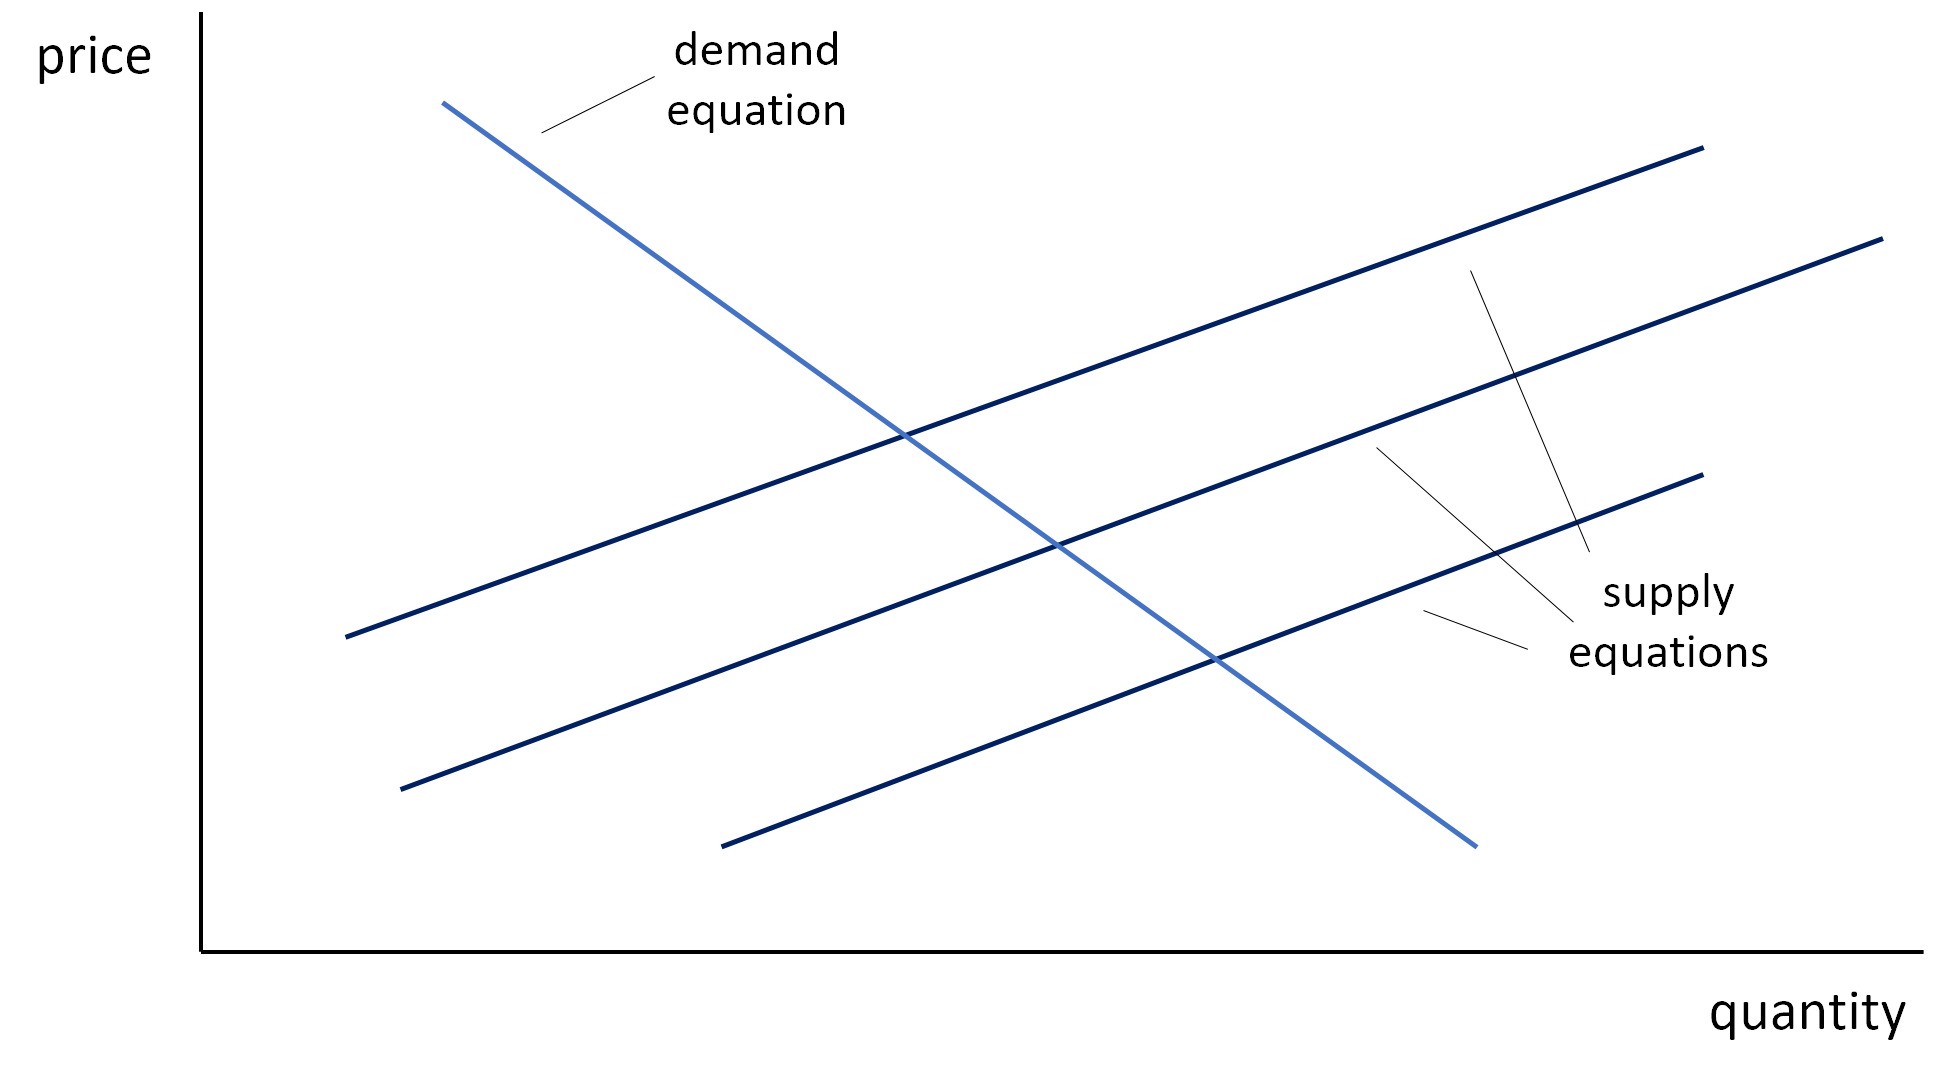
\includegraphics[width=\textwidth]{./img/W9_Obrazek_1}
\end{frame}
%---------------------------------------------
\section{Identification conditions}
\begin{frame}{Identification conditions}
Identification conditions for a sample 2-equation SEM \\(individual $i$ subscripts omitted)\\
\vspace{0.3cm}
\qquad $y_1 = \beta_{10} + \alpha_1 y_2 + \beta_{11} z_{11} + \beta_{12} z_{12} + \dots + \beta_{1k} z_{1k} + u_1$\\
\qquad $y_2 = \beta_{20} + \alpha_2 y_1 + \beta_{21} z_{21} + \beta_{22} z_{22} + \dots + \beta_{2k} z_{2k} + u_2$\\ 
\medskip
\begin{itemize}
\item  Order condition (necessary): $1^{st}$ equation is identified \\if at least one exogenous variable $z$ is excluded from $1^{st}$ equation (yet in the SEM).
\item Rank condition (necessary and sufficient): $1^{st}$ equation is identified if and only if the second equation includes at least one exogenous variable excluded from the first equation with a nonzero coefficient, so that it actually appears in the reduced form. 
\item For the second equation, the conditions are analogous.
\item Some estimation approaches allow for identification through IVs not explicitly included in the SEM.
\end{itemize}
\end{frame}
%---------------------------------------------
\begin{frame}{Examples}
\textcolor{Blue}{Example 4: (Identification)}\\ Labor supply of married working women\\
\bigskip
Supply (workers): 
\vspace{0.1cm}
\begin{flalign*}
\textit{hours} = \alpha_1 \log(\textit{wage}) & + \beta_{10} + \beta_{11} \textit{educ} + \beta_{12} \textit{age} + \beta_{13} \textit{kidslt}6 && \\
 & + \beta_{14} \textit{nwifeinc} + u_1 &&
\end{flalign*} \\
\medskip
Demand (enterprises):
\smallskip
\begin{flalign*}
\log(\textit{wage}) = & \alpha_2 \textit{hours} + \beta_{20} +\beta_{21} \textit{educ} + \beta_{22} \textit{exper} + \beta_{23} \textit{exper}^2 + u_2 && \\
\end{flalign*}
Order condition is fulfilled in both equations.
\end{frame}
%---------------------------------------------
\begin{frame}{Examples}
\textcolor{Blue}{Example 4: (Identification)}\\ Labor supply of married working women contnd.\\
\bigskip
\begin{itemize}
\item Identification of the first equation (Supply). For the rank condition, either $\beta_{22}$ or $\beta_{23}$ non-zero population coefficient (in the second equation) is required -- so that $\textit{exper},~\textit{exper}^2$ (or both) can be used in the reduced form.
\medskip
\item To evaluate the rank condition for supply equation, we estimate the reduced form for $\log(\textit{wage})$ and test if we can reject the null hypothesis that coefficients for both  $exper$ and $\textit{exper}^2$ are zero. \\If $H_0$ is rejected, the rank condition is fulfilled.\\
\medskip
\item We would do the evaluation of the rank condition for the demand equation analogically.
\end{itemize}
\end{frame}
%---------------------------------------------
\begin{frame}{Estimation}
\begin{itemize}
\item We can consistently estimate identified equations with the 2SLS method. \vspace{0.2cm}
\item In the $1^{st}$ stage, we regress each endogenous variable on all exogenous variables (``reduced forms'').
\vspace{0.2cm}
\item In the $2^{nd}$ stage we put into the structural equations instead of endogenous variables their predictions from the $1^{st}$ stage and estimate with the OLS method. 
\vspace{0.2cm}
\item The reduced form can be always estimated (by OLS).
\vspace{0.2cm}
\item In the $2^{nd}$ stage, we cannot estimate unidentified structural equations. 
\vspace{0.2cm}
\item With some additional assumptions, we can use a more efficient estimation method than 2SLS: 3SLS.
\end{itemize}
\end{frame}
%---------------------------------------------
\section{Systems with more than two equations}
\begin{frame}{Systems with more than two equations}
\textcolor{Blue}{Example 5:} Keynesian macroeconomic model
\vspace{0.2cm}
\begin{align*}
C_t & = \beta_0 + \beta_1(Y_t - T_t) + \beta_2 r_t + u_{t1} \\
I_t & = \gamma_0 + \gamma_1 r_t + u_{t2} \\
Y_t & \equiv C_t + I_t + G_t \\
\end{align*}
\vspace{-0.2cm}
\noindent Endogenous: $C_t, I_t, Y_t$ \hfill Exogenous: $T_t, G_t, r_t $ \\ 
\medskip
\begin{itemize}
\item Order condition for identification is the same as for two-equation systems, rank condition is more complicated. 
\item Complex models based on macroeconomic time series are sometimes used. Problems with these models: series are usually not weakly dependent, it is difficult to find enough exogenous variables as instruments. Question is, if any macroeconomic variables are exogenous at all.
\end{itemize}
\end{frame}
%---------------------------------------------
\begin{frame}{Identification in SEMs with more than two equations}
$\bm{y}_i = \bm{X}_i \bm{\beta}  + \bm{u}_i \qquad$ is the $i$-th equation of a SEM.\\
\medskip
$K$ - number of exogenous/predetermined variables in the SEM,\\ 
$K_i$ - number of $K$ in the $i$-th equation,\\
$G_i$ - number of endogenous variables in the $i$-th equation.\\
\bigskip
\textbf{Order condition} for the $i$-th equation:\\
necessary, not sufficient condition for identification\\
\bigskip
$K-K_i \geq G_i -1$\\
\bigskip
Condition evaluates as:
\begin{itemize}
\item[$=$] Equation $i$ is just-identified,
\item[$>$] Equation $i$ is over-identified,
\item[$<$] Equation $i$ is  not identified,\\
structural equation $i$ cannot be estimated by 2SLS/IVR.
\end{itemize}
\end{frame}
%---------------------------------------------
\begin{frame}{Identification in SEMs with more than two equations}
Rank condition: based on matrix algebra \& IV estimator\\
\medskip
Consider IVR for an identified $i$-th equation of SEM\\
\medskip
$\bm{y}_i = \bm{X}_i \bm{\beta} + \bm{u}_i$\\
\medskip
$\bm{X}_i$ is a $(n\! \times \! k)$ matrix, includes the intercept column and all endogenous regressors of the $i$-th equation,\\
\medskip
$\hat{\bm{X}}_i$ is a $(n\! \times \! k)$ matrix, includes the intercept column.\\
Exogenous regressors are repeated from $\bm{X}_i$, endogenous are projected to the column space of $\bm{Z}$: a $(n\! \times \! l)$ matrix of all exogenous variables in the SEM.\\
\bigskip
Single equation (limited information) estimator for each $i$-th equation:
\begin{itemize}
\medskip
\item $\hat{\bm\beta}_{\textit{IVR}} = \hat{\bm\beta}_{2\textit{SLS,i}}=
\left(\hat{\bm{X}}^{\prime}_i \bm{X}_i \right)^{-1}\! \hat{\bm{X}}^{\prime}_i \bm{y}$\\
\medskip
\item GMM -- moment equations can be used
\end{itemize}
\end{frame}
%---------------------------------------------
\begin{frame}{Identification in SEMs with more than two equations}
Rank condition: based on matrix algebra \& IV estimator (cont.)\\
\medskip
$\hat{\bm\beta}_{\textit{IVR}}=
\left(\hat{\bm{X}}^{\prime}_i \bm{X}_i \right)^{-1}\! \hat{\bm{X}}^{\prime}_i \bm{y}$\\
\bigskip
\begin{itemize}
\item \textbf{Order condition}: The necessary condition for the $i$-th equation to be identified is that the number of columns (exogenous variables of SEM) in $\bm{Z}$ should be no less than the number of columns (explanatory variables) in $\bm{X}_i$.\\
\medskip
\item \textbf{Rank condition}: The necessary and sufficient condition for identification of the $i$-th equation is that $\hat{\bm{X}}^{\prime}_i$ has full column rank of $\bm{X}_i$.\\
\dots ensures the existence of $\left(\hat{\bm{X}}^{\prime}_i \bm{X}_i \right)^{-1}$.
\end{itemize}
\end{frame}
%---------------------------------------------
\begin{frame}{Identification in SEMs with more than two equations}
Identification: recap \& final remarks\\
\bigskip
\begin{itemize}
\item Reduced form equations can always be estimated.\\
\smallskip
\item Structural equations can be estimated (IV/2SLS) \\only if identified: i.e. if rank condition is met.\\
\bigskip
\item With SW, checking rank condition for $\left(\hat{\bm{X}}^{\prime}_i \bm{X}_i \right)^{-1}$ is easy for finite datasets.\\
\smallskip
\item Asymptotic identification may be ``tricky'': \\because some columns in $\bm{X}_i$ are endogenous,\\
\smallskip
plim $n^{-1} \hat{\bm{X}}^{\prime}_i \bm{X}_i$ ~~ \\
\smallskip 
depends on the parameters of the DGP.\\
\medskip
\footnotesize{\dots see Davidson-MacKinnon (2009) Econometric theory and methods}
\end{itemize}
\end{frame}
%---------------------------------------------

\end{document}